\chapter{Évolution Différentielle}

\section{Introduction}

L'Évolution Différentielle (DE) est un algorithme évolutionnaire développé par Storn et Price \cite{Storn1995} en 1995. Il est versatile et relativement simple à implémenter et utiliser, ce qui en fait un outil essentiel dans toute boite à outils d'optimisation. Comme toutes les techniques évolutionnaires, le principe de l'évolution différentielle repose sur la génération d'une population de $N_P$ solutions (ou "vecteurs") qui permettent d'évaluer une fonction objectif à des points initiaux distribués aléatoirement dans un espace de recherche borné selon l'utilisateur. Ces points sont "perturbés" dans les générations successives de la population pour essayer de trouver des solutions extrémisant la fonction objectif. L'une des caractéristiques qui font la particularité de tout algorithme évolutionnaire est l'opération utilisée pour effectuer cette perturbation. Dans le cas de l'évolution différentielle, on perturbe une solution avec la différence de deux autres vecteurs de la population, multipliée par un facteur F, c'est l'opération dite de "mutation" comme est présenté dans la figure \ref{fig:deflowchart}. Ce nouveau vecteur subit une opération de croisement avec le vecteur initial pour produire le vecteur d'essai qui est comparé avec le vecteur de même indice dans la population. Ceci est refait jusqu'à ce que tous les vecteurs de la population soient comparés avec un vecteur d'essai (soit $N_P$ fois), créant la génération suivante. L'algorithme continue de créer de plus en plus de générations jusqu'à ce qu'un critère d'arrêt est satisfait. Souvent c'est un nombre de générations maximal ou une valeur de tolérance pour la variation de la fonction objectif.

\begin{figure}[H]
  \begin{center}
    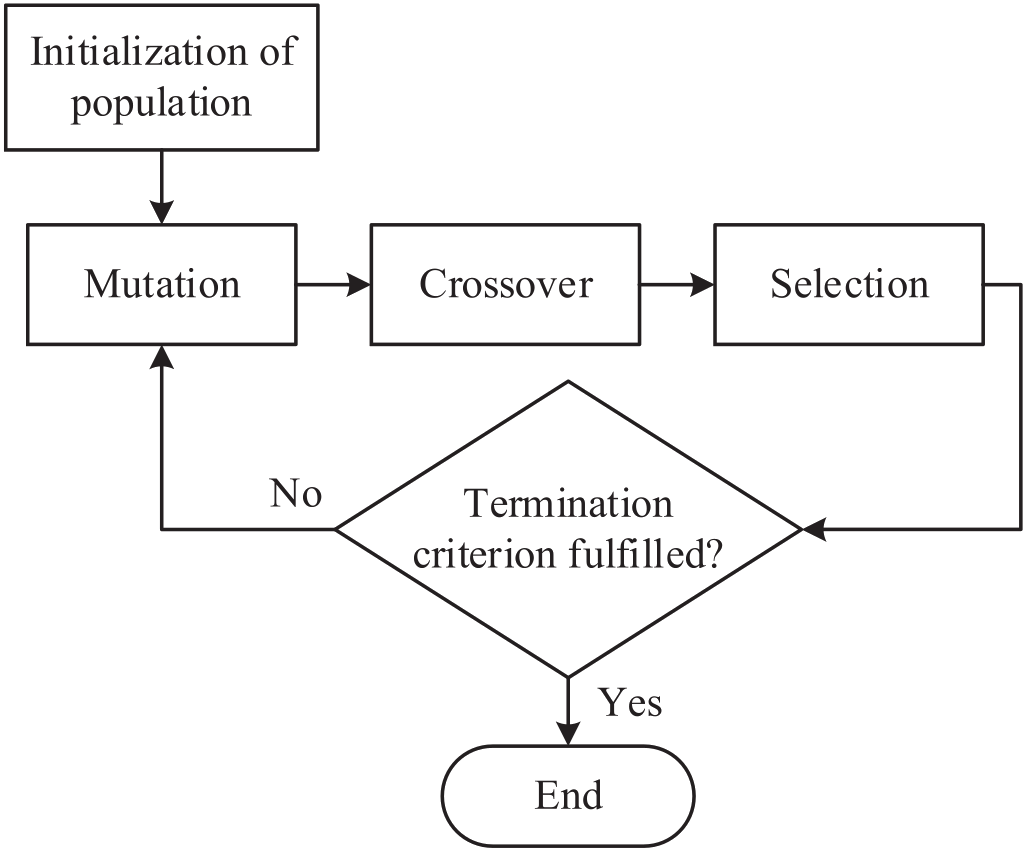
\includegraphics[width=.5\textwidth]{resources/DE.png}
    \caption{Organigramme des étapes de l'Évolution Différentielle}
    \label{fig:deflowchart}
  \end{center}
\end{figure}

\section{Description de l'algorithme}

\subsection{Initialisation}

\begin{wrapfigure}{r}{0.5\textwidth}
  \vspace*{-10pt}
  \begin{center}
    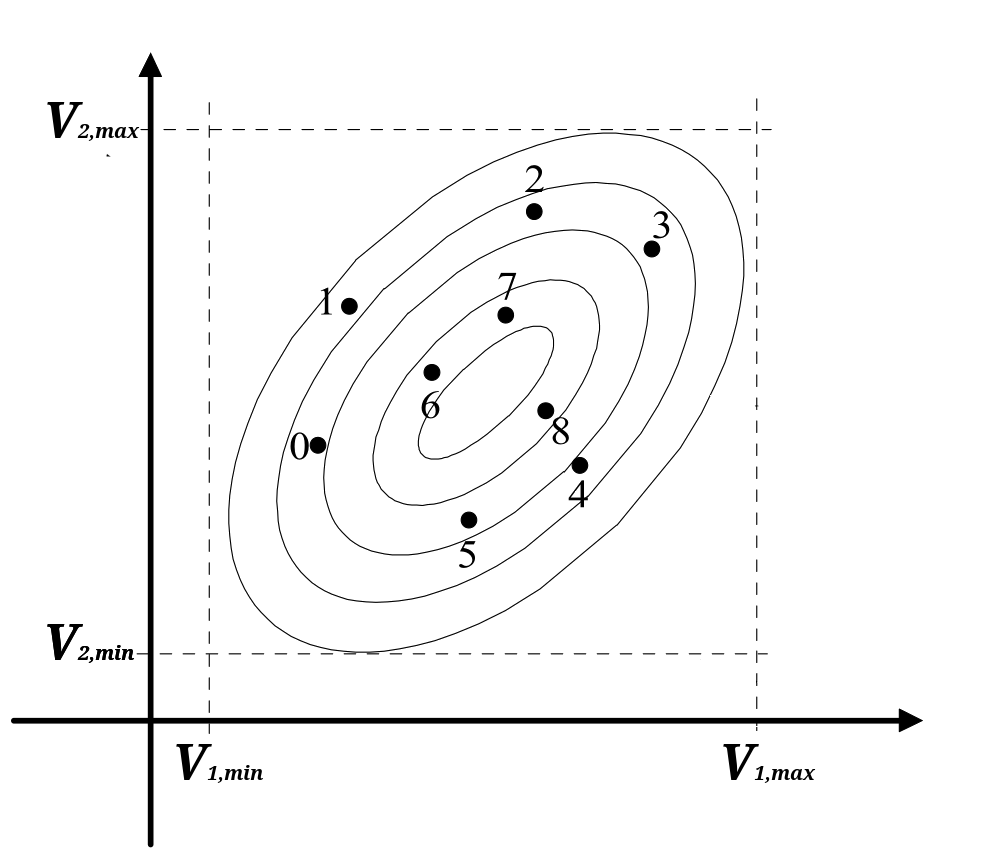
\includegraphics[width=\textwidth]{resources/initpop.png}
    \caption{Exemple d'une population initialisée dans un espace de recherche à deux dimensions donc dans ce cas $D = 2$, $N_P = 9$ }
    \label{fig:initpop}
        \vspace{30pt}
  \end{center}

\end{wrapfigure}

La convergence des techniques d'optimisation non-linéaire est toujours conditionnée par un "bon" choix des conditions initiales. Dans le cas de l'évolution différentielle, il s'agit de l'ensemble des vecteurs constituant la population initiale. Si un vecteur solution se constitue de $D$ paramètres, on travail avec un espace de recherche à $D$ dimensions, donc notre population initiale se compose de $N_P$ vecteurs à $D$ éléments. Mais pour pouvoir effectuer cette initialisation, les bornes de l'espace de recherche doivent être spécifiées. Chaque paramètre doit avoir une borne supérieure et inférieure, ce qui fait qu'on a besoin de $2 \times D$ valeurs pour spécifier complètement les bornes. Reste le mécanisme utilisé pour effectivement générer les vecteurs dans cet espace borné. Pour couvrir entièrement et uniformément cet espace, il faut, pour chaque paramètre de chaque vecteur, générer aléatoirement et uniformément une valeur comprise dans la fourchette déterminée. On utilise un générateur de nombres aléatoires. En considérant que l'indice $j$ associé à un vecteur $V_j$ désigne le $j-$ème paramètre, on peut accomplir ceci avec la formule \ref{eq:popinit}. 

\begin{equation}
  \label{eq:popinit}
  V_j = V_{\text{min},j} + \text{rand}[0, 1](V_{\text{max},j} - V_{\text{min},j})
\end{equation} 

On suppose avoir accès à une fonction $\text{rand}[0, 1]$, qui joue le rôle du générateur de nombres aléatoire uniformes et que $0 \leq \text{rand}[0, 1] < 1$. 
$V_{\text{min},j}$ et $V_{\text{max},j}$ sont les bornes inférieures   et supérieures du $j-$ème paramètres, respectivement. Figure \ref{fig:initpop} montre un exemple d'une population initialisée dans un espace de recherche 2 dimensionnel.

\subsection{Initialisation}

%\section{Application aux modèles simple et double diodes}

%\section{Métaheuristique}

 
